\documentclass[11pt, spanish, a4paper, twoside]{article}

% Versión 1.er cuat 2021 Víctor Bettachini < vbettachini@unlam.edu.ar >

\usepackage[T1]{fontenc}
\usepackage[utf8]{inputenc}

\usepackage[spanish, es-tabla]{babel}
% \def\spanishoptions{argentina} % Was macht dass?
% \usepackage{babelbib}
% \selectbiblanguage{spanish}
% \addto\shorthandsspanish{\spanishdeactivate{~<>}}


\usepackage{graphicx}
\graphicspath{{./figuras/}{../LaTeX/}{../figurasLaTeX/}}
% \usepackage{float}

\usepackage[arrowdel]{physics}
\newcommand{\pvec}[1]{\vec{#1}\mkern2mu\vphantom{#1}}
% \usepackage{units}
\usepackage[separate-uncertainty= true, multi-part-units= single, range-units= single, range-phrase= {~a~}, locale= FR]{siunitx}
\usepackage{isotope} % $\isotope[A][Z]{X}\to\isotope[A-4][Z-2]{Y}+\isotope[4][2]{\alpha}

\usepackage{tasks}
\usepackage[inline]{enumitem}
% \usepackage{enumerate}

\usepackage{hyperref}

% \usepackage{amsmath}
% \usepackage{amstext}
% \usepackage{amssymb}

\usepackage{tikz}
\usepackage{tikz-3dplot}
\usepackage{tikz-dimline}
\usetikzlibrary{calc}
% \usetikzlibrary{math}
\usetikzlibrary{arrows.meta}
\usetikzlibrary{snakes}
\usetikzlibrary{decorations}
\usetikzlibrary{decorations.pathmorphing}
\usetikzlibrary{patterns}

\usepackage[hmargin=1cm,vmargin=3cm, top= 0.75cm,nohead]{geometry}

\usepackage{lastpage}
\usepackage{fancyhdr}
\pagestyle{fancyplain}
\fancyhf{}
\setlength\headheight{28.7pt} 
\fancyhead[LE, LO]{\textbf{Mecánica Analítica Computacional} }
% \fancyhead[LE, LO]{\textbf{Mecánica General} }
\fancyhead[RE, RO]{\href{https://ingenieria.unlam.edu.ar/}{$\vcenter{\hbox{
\includegraphics[height=1cm]{ambos.pdf}}}$}}
\fancyfoot{\href{https://creativecommons.org/licenses/by-nc-sa/4.0/deed.es_ES}{$\vcenter{\hbox{
\includegraphics[height=0.4cm]{by-nc-sa_80x15.pdf}}}$} \href{https://ingenieria.unlam.edu.ar/}{DIIT - UNLaM}}
\fancyfoot[C]{ {\tiny Actualizado al \today} }
\fancyfoot[RO, LE]{Pág. \thepage/\pageref{LastPage}}
\renewcommand{\headrulewidth}{0pt}
\renewcommand{\footrulewidth}{0pt}



\begin{document}
\begin{center}
  % \textsc{\large Mecánica general}\\
  \textsc{\large Simulación de la dinámica | Resolución numérica de la ecuación de Euler-Lagrange}
\end{center}

\noindent
%De poder resolver estos problemas en forma autónoma puede asumir que adquirió los conocimientos mínimos sobre los temas abordados en la semana.
%No dude en consultar a docentes y compañeros si no puede terminarlos.
En los siguientes problemas resolverá numericamente cada ecuación de Euler-Lagrange que corresponda a cada coordenada generalizada.
Graficando tales soluciones, en el rango de tiempos y con las condiciones iniciales indicadas, estará simulando la dinámica de tales sistemas.\\
La aceleracion gravitatoria tiene por magnitud \(|\vec{g}| = \SI{9.81}{\metre\per\second\squared}\).\\
Los problemas marcados con (*) tienen alguna dificultad adicional, no dude en consultar.


\begin{enumerate}


\item 
\begin{minipage}[t][2.5cm]{0.7\textwidth}
\textbf{Máquina de Atwood simple}\\
Rango de tiempo \(t = \SIrange{0}{10}{\second}\).
Parámetros físicos y condiciones iniciales:\\
\(\ell_\mathrm{cuerda} > \SI{150}{\metre}\), 
\(R_{\mathrm{polea}\,1} = \SI{0.5}{\metre}\), \\ 
\(m_1 = \SI{8}{\kilo\gram}\), 
\(m_2 = \SI{1}{\kilo\gram}\), 
\(M_\mathrm{polea} = \SI{4}{\kilo\gram}\), \\
\(x(t=0) = \SI{25}{\metre}\), 
\(\dot{x}(t=0) = -\SI{10}{\metre\per\second}\).
\end{minipage}
\begin{minipage}[c][2cm][t]{0.3\textwidth}
	\hspace{0.5cm}
	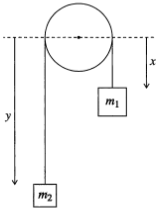
\includegraphics[width=0.6\textwidth]{marion_fig2_1a}
\end{minipage}



\item
	a) \textbf{Péndulo rígido ideal} [Marion (english) ex. 7.2] \\
	b) \textbf{Péndulo con punto de suspensión libre} [Landau \S5 ej. 2]\\ 
	c) \textbf{Péndulo doble} [Landau \S5 ej. 1] 
\begin{tasks}(3)
	\task \begin{tikzpicture}[scale= 1.0]
  	\draw [arrows=-latex] (-1,2) -> (-1,1) node [above=15, right=2] {\(\vec{g}\)}; % g vertical
		\draw [ultra thick] (-1.5,3) -- (2,3);
		\fill [pattern = north east lines] (-1.5,3) rectangle (2,3.2); % techo
		\draw [dashed] (0,3) -- (0,-.25);	% vertical
		\draw [thick] (0,3) -- +(-60:3) node[midway,above,right=2] {\(\ell\)};	% inclinada +:relativa, -60 grados, longitud 3
		\shade [ball color=black!80] ($(0,3)+(-60:3)$) circle(0.25) node [] {\color{white} $m$};
    \draw [arrows=-latex] (0,.4) -> (1.25,.4) node [midway, above] {\( \psi \)}; % desplazamiento horizontal
		\draw [arrows=-latex] (0,0) arc [start angle=-90, end angle=-65, radius=3] node [below=12, left=8] {\( \varphi \)};
	\end{tikzpicture}
	\task 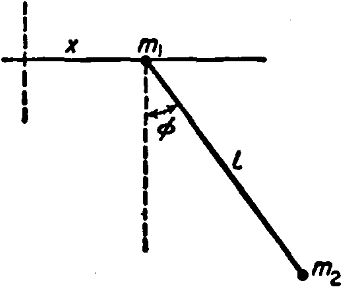
\includegraphics[height=0.2\textwidth]{landauS52_fig2}
	\task 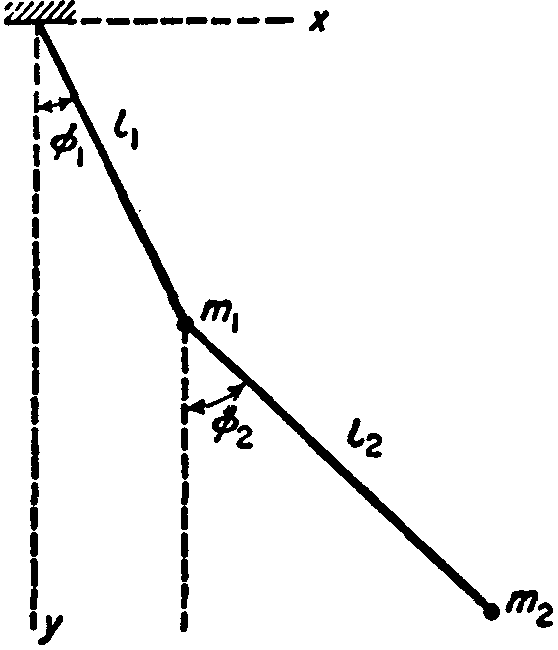
\includegraphics[height=0.2\textwidth]{landauS52_fig1}
\end{tasks}
Rango de tiempo \(t = \SIrange{0}{10}{\second}\).
Parámetros físicos y condiciones iniciales: 
\begin{enumerate}
	\item \(m = \SI{3}{\kilo\gram}\), 
				\(\ell = \SI{2}{\metre}\), 
				\(\varphi (t=0) = \frac{\pi}{4}\), \(\dot{\varphi} (t=0) = 0\).
	\item \(m_1 = \SI{3}{\kilo\gram}\), \(m_2 = \SI{1}{\kilo\gram}\),   
				\(\ell = \SI{2}{\metre}\), 
				\(x(t=0) = \SI{1}{\metre}\), \(\dot{x} (t=0) = \SI{0.5}{\metre\per\second} \),
				\(\phi (t=0) = \frac{\pi}{8}\), \(\dot{\phi} (t=0) = 0\).
	\item \(m_1 = \SI{3}{\kilo\gram}\), \(m_2 = \SI{1}{\kilo\gram}\),
				\(\ell_1 = \SI{1}{\metre}\), \(\ell_2 = \SI{1}{\metre}\),\\ 
				\(\phi_1 (t=0) = \frac{\pi}{8}\), \(\dot{\phi}_1 (t=0) = 0\), 
				\(\phi_2 (t=0) = \frac{\pi}{4}\), \(\dot{\phi}_2 (t=0) = -\frac{\pi}{16} \si{\per\second}\).
\end{enumerate}


\item 
	\begin{minipage}[t][2cm]{0.7\textwidth}
	\textbf{Péndulo de pesas engarzadas y acopladas}\\ 
	Rango de tiempo \(t = \SIrange{0}{10}{\second}\).
	Parámetros físicos y condiciones iniciales:\\
	\(m_1 = m_2 = m = \SI{2}{\kilo\gram}\), \(l = \SI{2}{\metre}\), \(\theta(t=0) = \frac{\pi}{4}\), \(\dot{\theta}(t=0) = 0\).
	\end{minipage}
	\begin{minipage}[c][2cm][t]{0.3\textwidth}
		\hspace{0.5cm}
  	 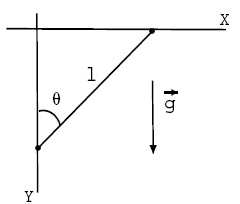
\includegraphics[width=0.6\textwidth]{fcen1-004}
	\end{minipage}



%\item \begin{minipage}[t][3.5cm]{0.6\textwidth}
%\textbf{Taylor ej. 7.2}
%Encuentre las ecuaciones de Euler-Lagrange para una partícula moviendose en dos dimensiones usando coordenadas polares.
%Asuma la presencia de una energía potencial \(V(r,\phi)\).
%\end{minipage}
%\begin{minipage}[c][1em][t]{0.35\textwidth}
%	\hspace{0.5cm}
%   \includegraphics[width=0.75\textwidth]{taylorFig7-1}
%\end{minipage}
%





\item
\begin{minipage}[t][2cm]{0.65\textwidth}
(*) \textbf{Maquina de Atwood compuesta} [Marion (english) ex. 7.8]\\ 
Rango de tiempo \(t = \SIrange{0}{5}{\second}\).
Parámetros físicos y condiciones iniciales:\\
\(\ell_\text{superior} = \SI{15}{\metre}\), 
\(R_{\text{polea sup}} = \SI{0.5}{\metre}\), 
\(\ell_\text{inferior} = \SI{15}{\metre}\), 
\(R_{\text{polea inf}} = \SI{0.5}{\metre}\),\\ 
\(m_1 = \SI{1}{\kilo\gram}\),
\(m_2 = \SI{2}{\kilo\gram}\),
\(m_3 = \SI{3}{\kilo\gram}\),
\(M_{\text{polea sup}} = \SI{4}{\kilo\gram}\),
\(M_{\text{polea inf}} = \SI{4}{\kilo\gram}\),\\
\(y(t=0) = \SI{1}{\metre}\), \(\dot{y}_1(t=0) = 0\),
\(y_2(t=0) = \SI{2}{\metre}\), \(\dot{y}_2(t=0) = 0\)
\end{minipage}
\begin{minipage}[c][3cm][t]{0.3\textwidth}
%	\begin{tikzpicture}
%		\draw [ultra thick] (-2,4) -- (2,4);
%		\fill [pattern = north east lines] (-2,4) rectangle (2,4.2); % techo
%		\draw (0,4) -- (0,3); % linea vertical techo - polea superior
%		\draw (0,3) circle [radius=0.5]; % polea superior
%		\draw (-0.5,3) -- (-0.5,1.5); % linea vertical izquierda polea sup - inf
%		\draw (0.5,3) -- (0.5,2.25); % linea vertical izquierda polea sup - m3
%		\draw (0.25,1.75) rectangle (0.75,2.25) node [anchor= north west] {\(m_3\)} ; % m3
%		% \draw (0.25,1.75) node [above=1, right=9.6] {\(m_3\)} rectangle (0.75,2.25) node [above=1, right=9.6] {\(m_3\)} ; % m3
%		\draw (-0.5,1.5) circle [radius=0.5]; % polea inferior
%		\draw (-1,1.5) -- (-1,.25); % linea vertical izquierda polea inf - m1
%		\draw (-1.25,-.25) rectangle (-0.75,0.25) node [anchor= north west] {\(m_1\)} ; % m1
%		\draw (0,1.5) -- (0,1); % linea vertical izquierda polea inf - m2
%		\draw (-.25,.5) rectangle (.25,1) node [anchor= north west] {\(m_2\)} ; % m2
%	\end{tikzpicture}
	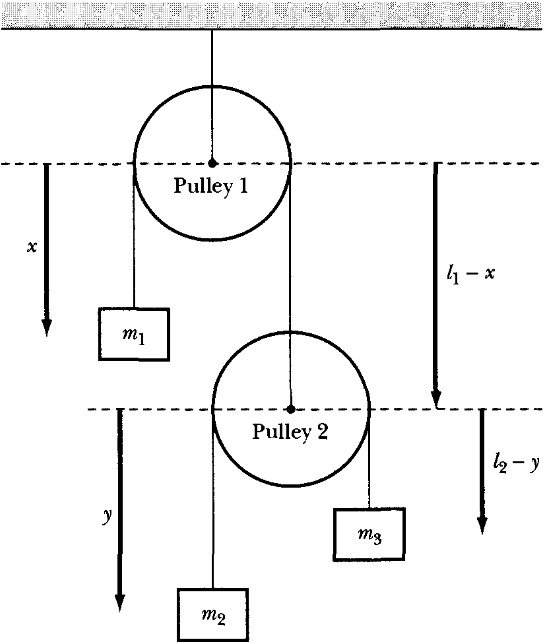
\includegraphics[width=\textwidth]{marion_fig7_6}
\end{minipage}




\end{enumerate}
\end{document}
